%% %% %% %%
%%
%% Previo de la práctica
%%
%% %% %% %%

\documentclass[../procedimientos.tex]{subfiles}
\graphicspath{{\subfix{../../images/}}}

\begin{document}
\subsection{Previo}
\subsubsection*{Pregunta 1}
\begin{em}
  ¿Qué es un cronograma?
\end{em}

Se trata de la representación gráfica de un conjunto de señales de entrada y 
salida como funciones del tiempo. Las señales son representadas en el eje de 
las ordenadas, y el tiempo en el de las abscisas, reflejando mediante la 
gráfica la evolución o estado de la señal en cada instante de tiempo. Debido a 
que dichas señales pueden tomar únicamente valores de $0$ y $1$, su 
representación gráfica es una serie de pulsos cuadrados con diferentes 
longitudes. Las señales de entrada y salida se dibujan en el mismo diagrama 
para mostrar el comportamiento entrada-salida del sistema digital. Un 
cronograma muestra todos los posibles patrones de entrada-salida (tal como lo 
hace la tabla de verdad).

\subsubsection*{Pregunta 2}
\begin{em}
  ¿Qué son las señales tipo Toggle, Random y Pulse?
\end{em}

\begin{itemize}
  \item \textbf{Toggle.} El término \textit{toggle} hace referencia a que 
  existe una conmutación; es decir, se trata de una señal que sólo puede tomar 
    dos valores, cada uno de los cuales representa un estado lógico. La señal 
    de tipo toggle se genera a partir de un dispositivo \textit{flip-flop} 
    (conformado por compuertas lógicas), el cual recibe una señal de reloj y 
    una señal digital $T$; esta última determina la forma que tendrá la señal 
    \textit{Toggle}, si $T=0$, la señal \textit{Toggle} mantiene su valor 
    anterior hasta el siguiente ciclo de reloj; caso contrario, si $T=1$, la 
    señal invierte su valor.
  \item \textbf{Random.} Se trata de una señal que puede adquirir cualquier 
    valor para cualquier tiempo dado; es decir, se genera a partir de valores 
    aleatorios. No existe algún patrón que se repita en ella, de hecho, 
    presenta muchas fluctuaciones y no se pueden modelar con alguna función 
    matemática.
  \item \textbf{Pulse.} Se trata de una señal que toma un valor determinado 
    (estado de encendido) durante un tiempo finito, denominado tiempo 
    \textit{on}, y toma un valor de $0$ (estado de apagado) durante un tiempo 
    off, también finito; la suma del tiempo \textit{on} y el tiempo 
    \textit{off} es el periodo de la señal (denotado por $T$). El 
    comportamiento anterior se repite a lo largo del tiempo para generar la 
    señal; por lo que, ésta se encuentra conmutando entre su estado inicial y 
    el complemento de este.
\end{itemize}

\subsubsection*{Pregunta 3}
\begin{em}
  ¿Para qué se utiliza la resistencia Pull-Up o Pull-Down?
\end{em}

Se trata de resistencias dispuestas en un circuito de forma especial con la 
finalidad de mantener un estado lógico de manera estable en la entrada del 
circuito; es decir, para evitar posibles perturbaciones derivadas de señales 
de ruido.
\begin{itemize}
  \item \textbf{Resistencia Pull Down.} En esta configuración, la resistencia 
    tendrá una caída de potencial de $0 [V]$ de forma predeterminada 
    (\textit{LOW}), ya que un extremo de la resistencia se conecta 
    directamente a Tierra, reflejándose en el otro extremo; mientras que 
    tendrá una caída de potencial de $V_{CC}$ en caso contrario 
    (\textit{HIGH}), si el extremo de la resistencia se conecta directamente a 
    $V_{CC}$, disipando toda la tensión.
  \item \textbf{Resistencia Pull Up.} En esta configuración, la resistencia  
    tendrá una caída de potencial de $V_{CC}$ de forma predeterminada 
    (\textit{HIGH}); es decir, el voltaje $V_{CC}$ conectado al otro extremo 
    de la resistencia se ve reflejado; mientras que tendrá una caída de 
    potencial de $0[V]$ en caso contrario (\textit{LOW}); es decir, en caso de 
    que la resistencia se conecte directamente a Tierra.
\end{itemize}

\begin{figure}[H]
  \centering
  \begin{subfigure}[b]{0.45\textwidth}
    \centering
    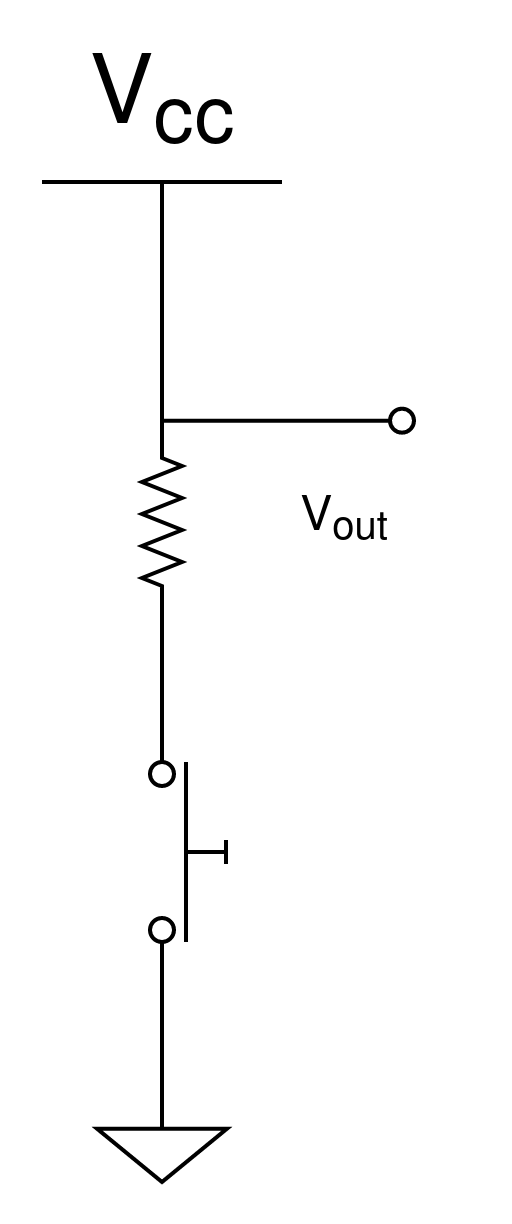
\includegraphics[height=7cm]{pull_down}
    \subcaption{\textit{Pull Down}}
  \end{subfigure}
  \hfill
  \begin{subfigure}[b]{0.45\textwidth}
    \centering
    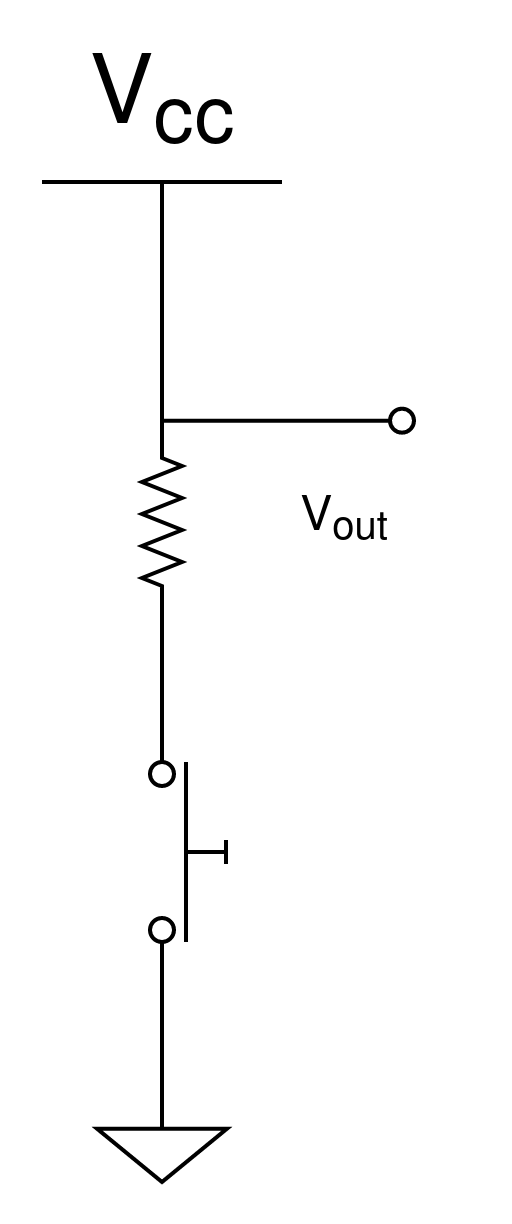
\includegraphics[height=7cm]{pull_up}
    \subcaption{\textit{Pull Up}}
  \end{subfigure}
  \caption{Resistencias \textit{Pull Up} y \textit{Pull Down}}
\end{figure}

\subsubsection*{Pregunta 4}
\begin{em}
  ¿Para un transistor a qué se le llama ``Corte'' y ``Saturación'' y cuál es su 
  efecto sobre las señales lógicas?
\end{em}

Se trata de dos regiones de operación de los transistores.
\begin{itemize}
  \item \textbf{Corte.} Un transistor está en corte cuando las uniones que lo 
    conforman están polarizadas en sentido inverso, lo cual produce una 
    corriente de colector despreciable y por ende, también la corriente a 
    través de la terminal emisora es despreciable. En este caso, el transistor 
    se comporta como un interruptor abierto.

  \item \textbf{Saturación.} Un transistor está en saturación cuando las 
    uniones que lo conforman están polarizadas en directa, lo cual genera un 
    crecimiento exponencial de la corriente que circula a través de su 
    terminal colector, y en consecuencia, a través de la terminal emisora. En 
    este punto el transistor actúa como un interruptor cerrado, permitiendo el 
    paso de la corriente.
\end{itemize}

Abstrayendo el comportamiento descrito, se puede considerar un estado 
\textit{on} cuando el transistor está en la región de saturación y un 
\textit{off} cuando el transistor está en la región de corte.

\subsubsection*{Pregunta 5}
\begin{em}
  Analiza y caracteriza el siguiente circuito a través de cualquier simulador 
  e identifica el comportamiento que este tiene.
  \begin{itemize}
    \item Identifica el voltaje resultante en cada uno de los transistores 
      considerando que tanto la entrada A como B solamente pueden tener dos 
      voltajes (ground y $V_{CC}$), toda esta información colócala dentro de 
      una respectiva tabla y completa la misma.
  \end{itemize}
\end{em}

Para este caso, dentro del simulador se consideró un voltaje $V_{CC} = 5 [V]$, 
con lo cual se obtuvieron los siguientes valores:

\begin{table}[H]
  \centering
  \scalebox{0.8}{
    \begin{tabular}{|p{1.5cm}|p{1.5cm}|p{1.5cm}|p{1.5cm}|p{1.5cm}|p{1.5cm}|}
      \hline
      \textbf{A}& \textbf{B}& \textbf{C}& \textbf{Q1}& \textbf{Q4}& \textbf{Q2, Q3}  \\ \hline
      Ground  & Ground  & Ground  & 2.8     & 2.8     & 0       \\
      Ground  & Ground  & VCC     & 2.8     & 0       & 0       \\
      Ground  & VCC     & Ground  & 0       & 2.8     & 0       \\
      Ground  & VCC     & VCC     & 0       & 0       & 5       \\
      VCC     & Ground  & Ground  & 0       & 2.8     & 0       \\
      VCC     & Ground  & VCC     & 0       & 0       & 5       \\
      VCC     & VCC     & Ground  & 0       & 2.8     & 0       \\
      VCC     & VCC     & VCC     & 0       & 0       & 5       \\ \hline
    \end{tabular}
  }
  \caption{Voltajes de la simulación (Pregunta 5)}
\end{table}

La simulación se llevó a cabo en lal plataforma \textit{Qucs}, tal como se 
muestra a continuación:
\begin{figure}[H]
  \centering
  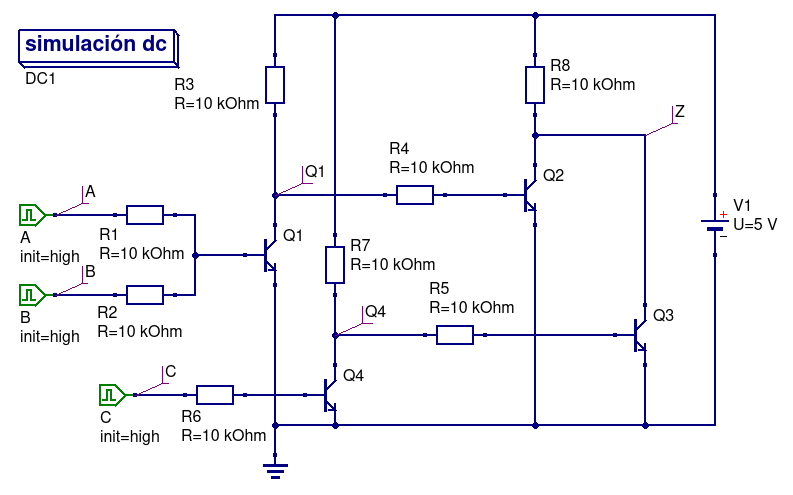
\includegraphics[width=10cm]{previo_simulacion}
  \caption{Circuito de simulación en \textit{Qucs} (Pregunta 5)}
\end{figure}

La caracterización de la configuración de cada uno de los transistores es la 
siguiente:
\begin{itemize}
  \item $Q_1$: $f_1(ABC) = \nt{A}\nt{B}\nt{C} + \nt{A}\nt{B}C$
  \item $Q_4$: $f_4(ABC) = \nt{A}\nt{B}\nt{C} + A\nt{B}C+A\nt{B}\nt{C} + 
    A\nt{B}C + AB\nt{C}$
  \item $Q_2, Q_3$: $f_{2,3}(ABC) = \nt{A}BC + A\nt{B}C + ABC$

\end{itemize}

\end{document}

